\documentclass[12pt,letterpaper,english,bibliography=totocnumbered, abstract=on]{scrartcl}

\usepackage{indentfirst}
\usepackage[titletoc]{appendix}
\usepackage[T1]{fontenc}
\usepackage[latin9]{inputenc}
\usepackage{color}
\usepackage{babel}
\usepackage{verbatim}
\usepackage[unicode=true,pdfusetitle,
bookmarks=true,bookmarksnumbered=false,bookmarksopen=false,
breaklinks=true,pdfborder={0 0 0},pdfborderstyle={},backref=false,colorlinks=true]
{hyperref}
\hypersetup{linkcolor=blue,citecolor=blue,urlcolor=blue}

\usepackage{booktabs}
\usepackage{multirow}
\usepackage{adjustbox}
\usepackage{threeparttable}
\usepackage[table]{xcolor}
\usepackage{csquotes}
\usepackage{soul} % for hiliting text: \hl

\usepackage[backend=biber, style=authoryear, maxbibnames=99, dashed=false]{biblatex}
\setlength\bibitemsep{2\itemsep}
\addbibresource{CRB.bib}

\usepackage{pdfpages}
\usepackage{float} % Allows use of H to place floats

\usepackage{pgfgantt}

\usepackage{framed}

% Prevent page breaks within paragraphs
% https://tex.stackexchange.com/questions/21983/how-to-avoid-page-breaks-inside-paragraphs
\widowpenalties 1 10000

\begin{document}

\titlehead{Request for Interest}

\title{Object Detector(s) for Quantification of Coconut Rhinoceros Beetle Damage in Roadside Video Surveys}

\author{Aubrey Moore PhD, Entomologist, University of Guam\\
	aubreymoore@guam.net | cell 1-671-686-5664 | UTC+10h}

\date{June 3, 2020}

\maketitle


\begin{figure}[h]
	\centering
	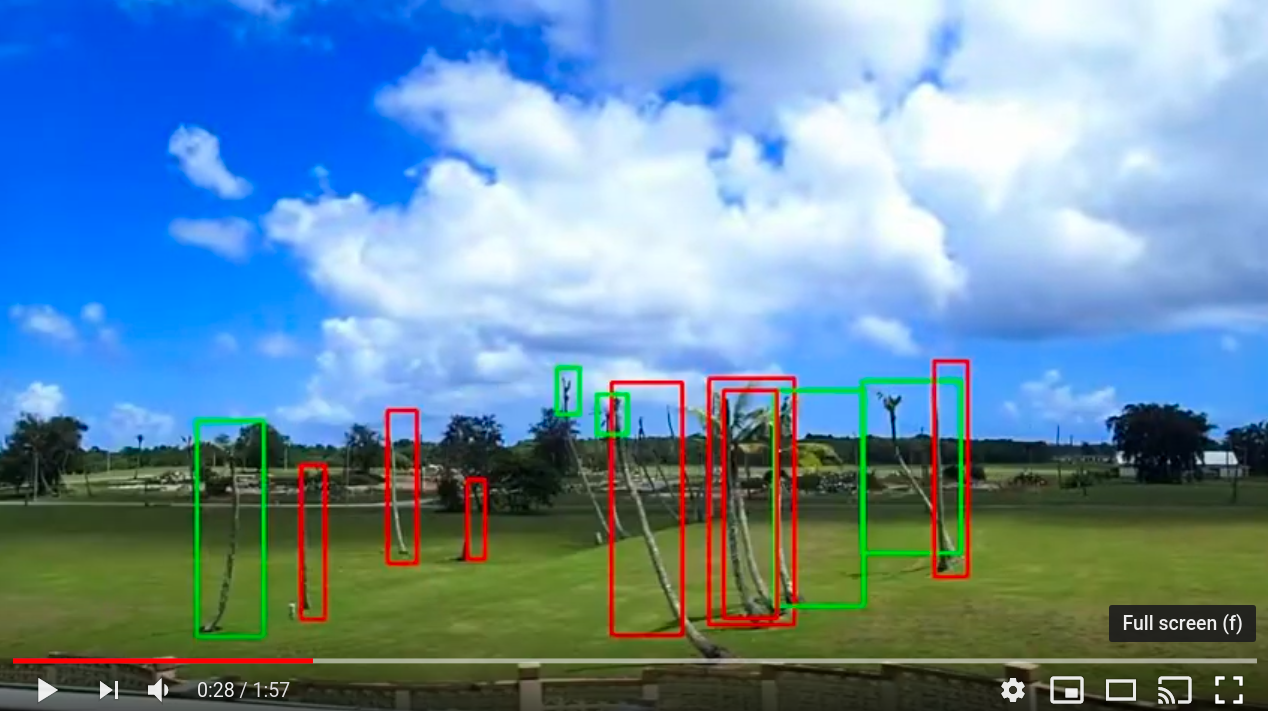
\includegraphics[width=0.7\linewidth]{images/royal-palms}
	\caption{Training an Object Detector to Locate Coconut Palms Damaged or Killed by Coconut Rhinoceros Beetle. Please view the video at \url{https://youtu.be/zzSorqcmt9U}. Result of a first attempt to train an object detector (Faster R-CNN) to locate coconut trees killed or damaged by coconut rhinoceros beetle in a video. Dead palms are in red boxes, damaged palms are in green boxes. Not perfect, but it does serve as a proof of concept.}
	\label{fig:royal-palms}
\end{figure}

This RFI is intended to identify qualified entities with skills in computer vision and machine learning which may be interested in collaborating on development of an automated system which uses image analysis of roadside video surveys to detect and quantify coconut rhinoceros beetle damage in images collected during roadside video surveys. Financial support for this project has been granted with a fixed completion date of July 31, 2020.

If you are interested in a contract to develop the object detector(s) required by this project, please contact Dr.Aubrey Moore before June 10, 2020.

\section{Background} 

Coconut palms on several Pacific Islands are being damaged and killed by outbreaks of coconut rhinoceros beetle (CRB). Damage is done when an adult beetle bore into the crown to feed on sap. Fronds developing within the crown are damaged when the beetle bores through them. This damage becomes evident as distinctive v-shaped cuts when these fronds emerge and unfurl (Fig. \ref{fig:dying-coconuts}). If the bore hole passes through the meristem (the growing tip), the palm may be mortally wounded, losing the ability to generate additional fronds. Mortally wounded palms eventually die when existing fronds senesce and fall off, leaving a dead, standing trunk (Fig. \ref{fig:royal-palms}, \ref{fig:dying-coconuts}).

There is a need to monitor CRB damage for two reasons:
\begin{itemize}
	\item to measure changes in time and space, especially changes in response to control activities, on islands infested with CRB
	\item early detection of CRB damage on newly invaded islands
\end{itemize}
In the past, CRB damage surveys have been performed by direct observation by skilled individuals. We propose that this work can be automated by digital analysis of roadside videos collected by dash cams.  

\section{System Design}

\subsection{Prototype System}

A prototype system was developed as a proof-of-concept. A roadside video of damaged and dead coconut palms was recorded using a digital camera (Olympus TG-5) hand held looking out of the passenger window of a moving car. CVAT was used to annotate the first half of the video by drawing labeled bounding boxes around damaged and dead coconut palms. Images in these bounding boxes were used to train a Faster R-CNN model). Frames in the in the last half of the video were used as a test set (See Fig. \ref{fig:royal-palms} and associated YouTube video). 

\subsection{Operational System}

\begin{description}
	
	\item[Video capture.] A smart phone (Samsung Galaxy 10) running a dash cam app (Road Recorder) will be used for roadside video capture. The app uses the phone's GPS receiver to log camera position during the video. Roadside videos will be recorded on microSD cards.
	
	\item[Object Detection.] One or more object detectors will be designed and trained to count the number of healthy coconut palms, CRB-damaged coconut palms (indicated by v-shaped cuts) and dead coconut palms (dead, standing trunks) in each video frame.	
	For training purposes, roadside videos will initially be uploaded from microSD cards to an internet repository. When object detectors are operational, they will probably be run on a local machine eliminate the necessity of uploading large files to an internet server. 
	
	\item[Output Data] Output data will include camera location, time stamp, and number of coconut palms visible in each frame classified into three damage levels (healthy, damaged, dead). Reports containing maps will be developed to visualize these data.
	
\end{description}

\section{Requirements}

\begin{itemize}
	
	\item The system must be built using free open-source software (FOSS).  Preferred components include Linux, OpenCV, Python, Jupyter and CVAT.
	
	\item The system should be designed so that it can be operated locally in early detection mode on remote Pacific Islands which do not have access to modern telecommunications networks. Distribution of turnkey systems on Raspberry Pis would be ideal. 
	
\end{itemize}

\section{Deliverables}

\begin{itemize}
	
	\item Fully trained and tested object detector(s) capable of detecting all coconut palms classified into three mutually exclusive groups:
	
		\begin{itemize}
			\item healthy coconut palm (no CRB damage [Fig. \ref{fig:healthy}]) 
			\item CRB-damaged coconut palm (indicated by v-shaped cuts [Fig. \ref{fig:dying-coconuts}])
			\item dead coconut palm (dead standing trunk [Fig. \ref{fig:dying-coconuts}])
		\end{itemize}
		
	\item A comprehensive report containing:
	
	\begin{itemize} 
		\item complete documentation including a validation report for the object detector(s) and all source code

		\item suggested parameters for operational video survey recording (optimal frame size, minimum frame rate, etc.)
	\end{itemize}

\end{itemize}

\begin{figure}[]
	\centering
	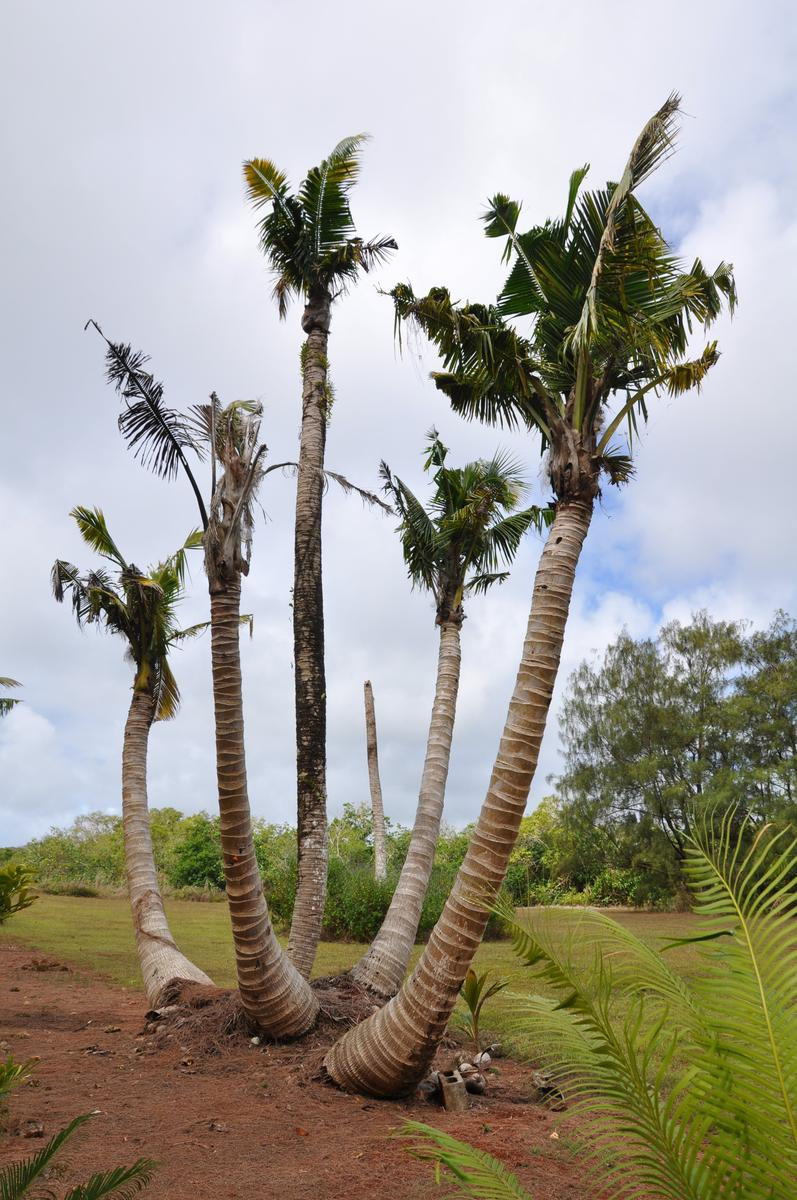
\includegraphics[width=0.7\linewidth]{images/dying-coconuts.png}
	\caption{Coconut palms damaged by coconut rhinoceros beetle (indicated by v-shaped cuts). Also, a dead, standing trunk in background.}
	\label{fig:dying-coconuts}
\end{figure}

\begin{figure}[]
	\centering
	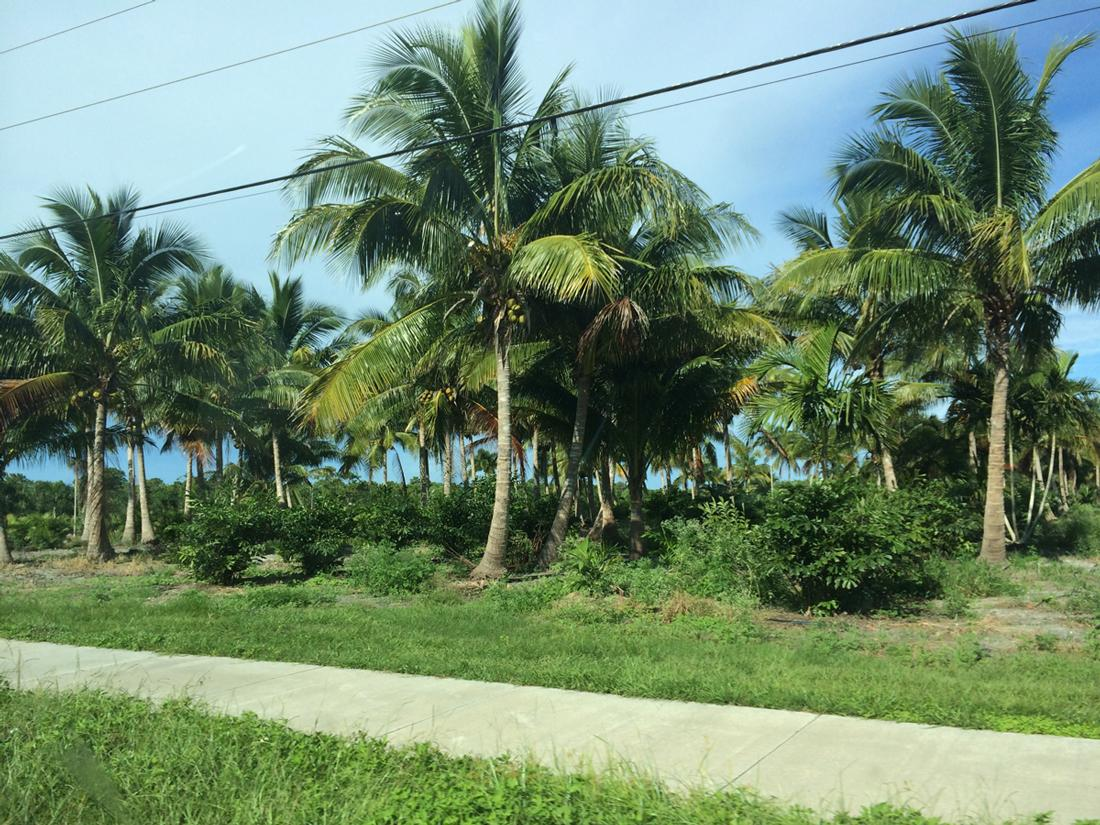
\includegraphics[width=0.7\linewidth]{images/healthy.jpg}
	\caption{Healthy coconut palms.}
	\label{fig:healthy}
\end{figure}


 

%\newpage
%\tableofcontents
%\pagebreak
%
%\section{Section}
%
%\newpage{}
%\begin{appendices}
%	
%\section{Form SF-424}
%Please see next page.
%\includepdf[pages=-]{forms/SF424-signed.pdf}
%
%\end{appendices}

\end{document}
